% !TEX root = ../main.tex
\chapter{Implementation}
\label{Implementation}
In this section, how the design is implemented will be described in detail

\section*{Agents}
Agents in Presage 2 are created by extending the AbstractParticipant class. As Virtual Agents and Prosumer Agents behave in a similar fashion, the Prosumer Agent is designed to extend the Virtual Agent with additional properties such as ParentID and ability to add Demand/Generation profiles.

\begin{figure}[!h]
	\centering
	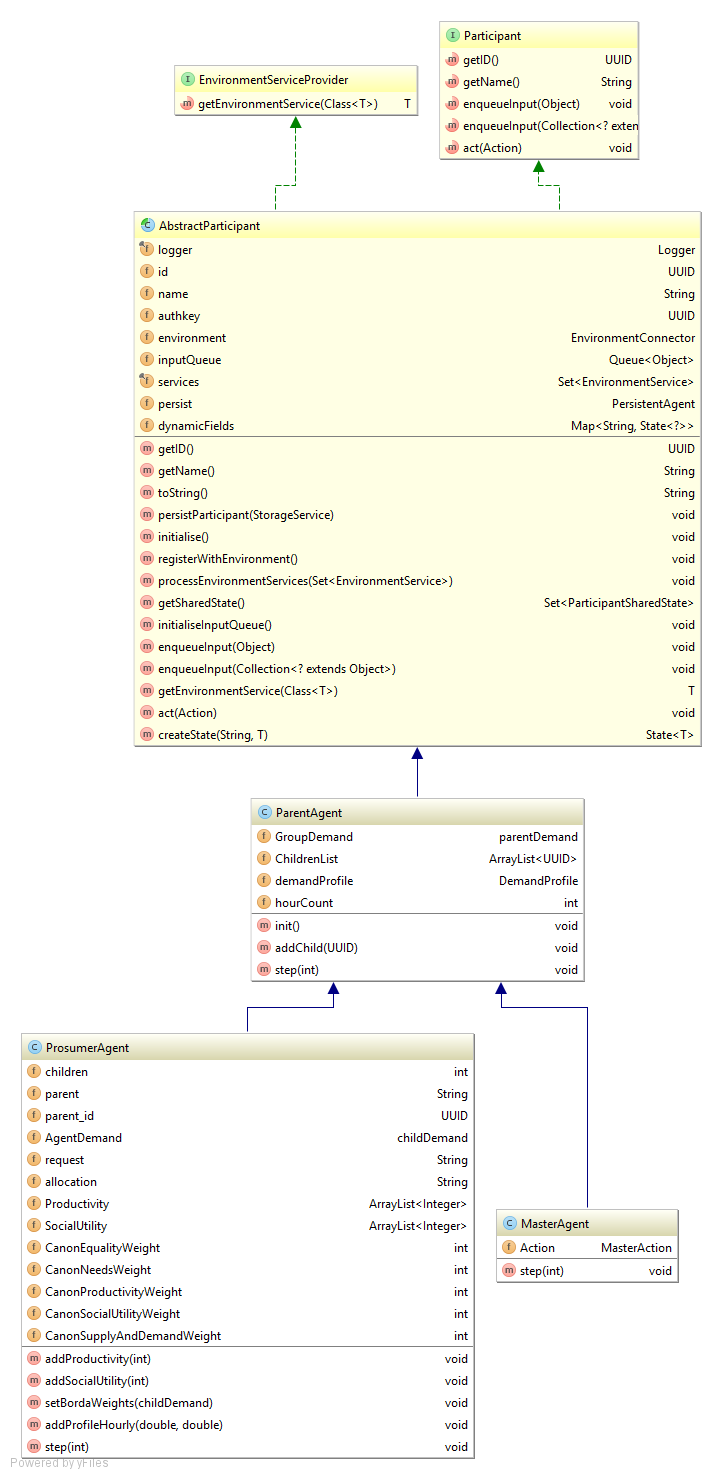
\includegraphics[scale=0.71]{Images/AgentUML.png}
	\caption{Agent UML Diagram}
	\label{fig:AgentUML}
\end{figure}

\section*{Environment Services}
All Agents act within Environments, which would contain shared state between Agents. In the context of this simulation shared state would be information such as the amount available in the Common Resource Pool.

\begin{figure}[!h]
	\centering
	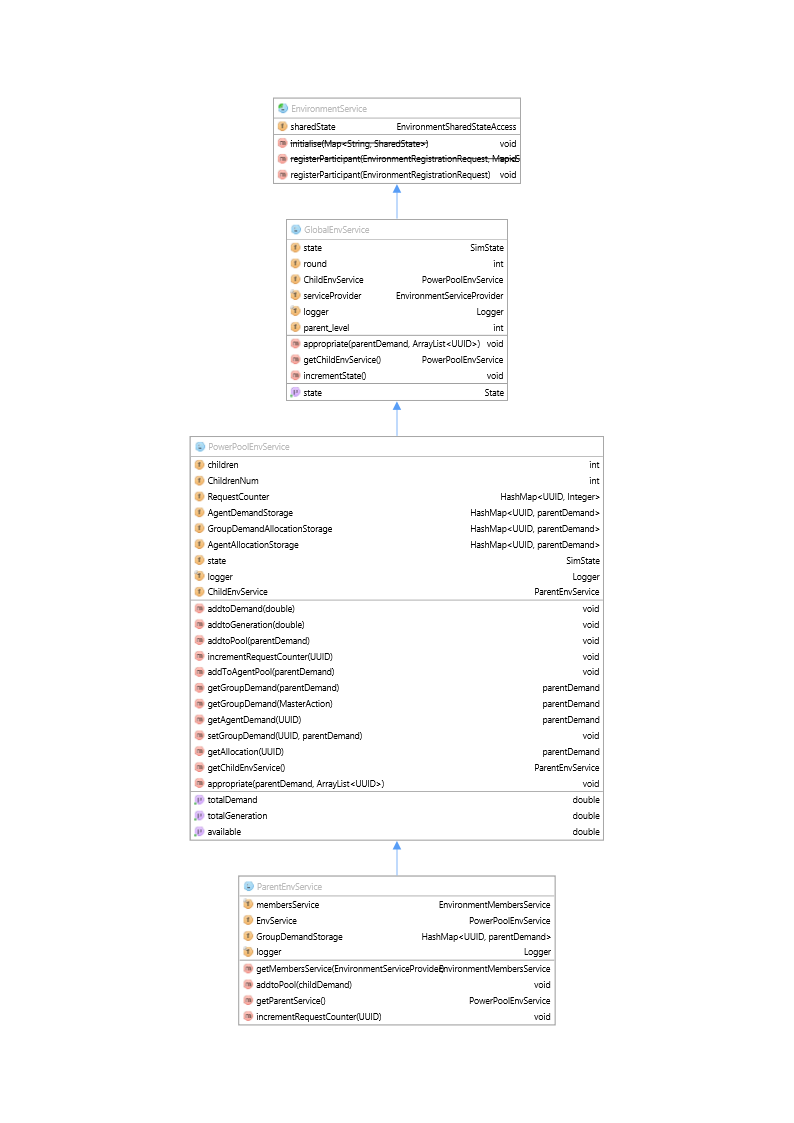
\includegraphics[scale=0.71]{Images/EnvironmentUML.png}
	\caption{Environment Services UML Diagram}
	\label{fig:ServiceUML}
\end{figure}

\subsection*{Action}
To act on the Environment or acess a shared state in the Environment, Agents are expected to perform an Action. In the context of this simulation, Action would be Demand/Generation requests. As Generation can be modelled as a negative Demand, a single Action can be defined to allow the contribution and appropriation of electricity. 

\begin{figure}[!h]
	\centering
	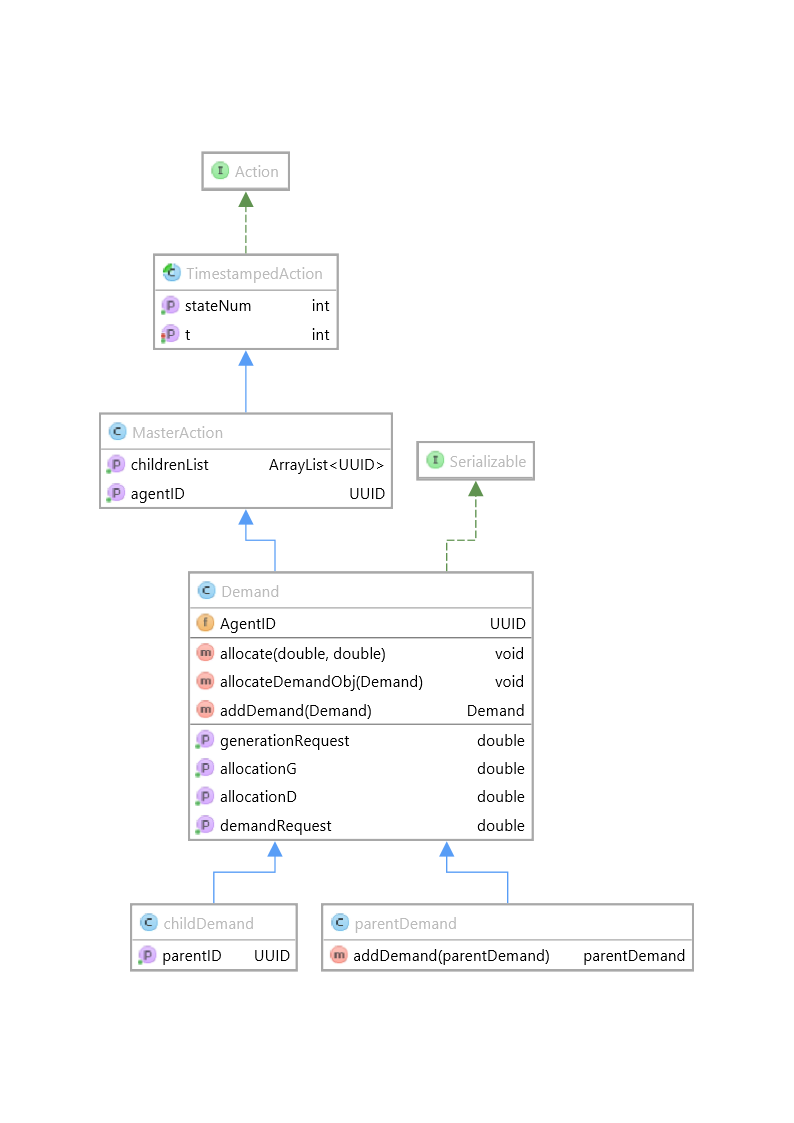
\includegraphics[scale=0.5]{Images/ActionUML.png}
	\caption{Actions UML Diagram}
	\label{fig:ActionUML}
\end{figure}

\subsection*{Action Handlers} % (fold)
To enable the Environment to be able to process the Action requests, Action Handlers need to be created to tell the simulation how to deal with Actions from Agents.

\begin{figure}[!h]
	\centering
	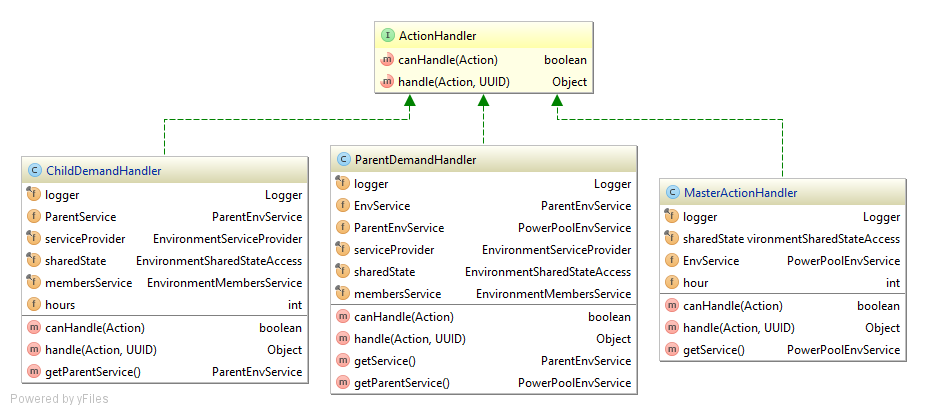
\includegraphics[scale=0.4]{Images/ActionHandlerUML.png}
	\caption{Action Handler UML Diagram}
	\label{fig:ActionHandlerUML}
\end{figure}
% subsubsection subsubsection_name (end)

\subsection*{Simulation}


\section*{Issues}
Out of order parallel execution meant that Agents need to submit their individual Demands to the SharedState, and have that summed at the end of each timestep. It is not possible to sum the Demands on the fly.

Being new to both Java and Presage presented problems of its own. It was difficult to understand how simulations could be run and therefore create our own.

One action per time step meant that it takes 4 time steps to simulate one round of request and appropriation of electricity. It would therefore take 24*4 time steps to simulate a full day of requests and appropriation.
